%
% pef.tex (LateX)
% 
% Objetivo: Capítulo sobre o método de interpolação com filtros adaptativos de predição de erro
% (PEF, do inglês) do relatório de qualificação de doutorado.
% 
% Versão 1.0
% 
% Site: http://www.dirackslounge.online
% 
% Programador: Rodolfo A. C. Neves (Dirack) 17/10/2019
% 
% Email: rodolfo_profissional@hotmail.com
% 
% Licença: GPL-3.0 <https://www.gnu.org/licenses/gpl-3.0.txt>.

\chapter{FILTROS ADAPTATIVOS DE PREDIÇÃO DE ERRO (FPE)}

Uma restrição comumente utilizada na interpolação de traços sísmicos
é assegurar que os dados interpolados, depois da filtragem,
tenham mínima energia. Isto significa a escolha de valores
nos limites do filtro de modo a minimizar o transiente. Neste ponto os mínimos
quadrados levam grande vantagem, pois tendem a absorver grandes valores e a distribuir
uniformemente os resíduos em tempo e frequência na extensão permitida \cite{claerbout92}.

A filtragem é equivalente a multiplicação espectral. Assim, especificar a filtragem
é o equivalente a preescrever o espectro dos dados interpolados. Uma escolha sensível
é o espectro do dado registrado, que pode ser capturado através dos coeficientes dos
filtros adaptativos de predição de erro (FPE) do dado \cite{spitz}. 

Os FPE, também conhecidos como filtros de autoregressão, desenpenham o
papel da ``matriz inversa de covariância'' da teoria das estimativas na estatística.
O sinal é regredido sobre si mesmo na estimativa dos coeficientes do filtro. O FPE
pode ser implementado na domínio tempo-espaço ou frequency-espaço. FPE no tempo-espaço
são menos propensos a criar eventos espúrios na presença de ruído do que os filtros
frequência-espaço \cite{abma}. 

A utilização dos FPE na interpolação ocorre em dois passos:
Primeiro, o FPE é estimado através da minimização da saída da convolução
dos dados conhecidos com o FPE desconhecido. Segundo, os dados interpolados
são estabelecidos a partir da minimização da convolução do FPE anteriormente 
calculado com o modelo conhecido, restringido pelos dados conhecidos. \cite{curry}.

Os filtros adaptativos de predição de errro (FPE) podem ser utilizados para regularizar os dados sísmicos,
de modo a produzir uma amostragem suficiente para o estabelecimento das seções ERC.
Como representado na Figuras \ref{fig:3.1}, a trajetória ERC calculada para cada $m_0$ não
necessariamente intersecta as seções de afastamento constante nas coordenadas $m_i$, $h_i$ dos traços sísmicos. 
A trajetória ERC calculada passa entre os traços identificados pelas coordenadas $m1,h2$ e $m3, h2$ na Figura \ref{fig:3.1},
sendo necessário aumentar a discretização da seção $h2$ para poder amostrar corretamente a trajetória ERC.

Ao intercalar os traços originais com novos traços zerados $m'_i$, e utilizar os filtros adaptativos de predição
de erro para interpolar os valores das amostras em cada traço $m'_i$, dobramos 
a discretização das seções de afastamento constante.
Este processo pode ser repetido até que a discretização seja suficiente para amostrar a curva ERC em cada seção de afastamento
constante (na Figura \ref{fig:3.2}, $m'_2$ está mais próximo da trajetória 
ERC do que $m_3$ e $m_2$ já que a distância 
entre os traços da seção $\Delta h$ é menor).

\begin{figure}
\caption{Representação esquemáticas de uma trajetória ERC para um $m_0$ arbitrário. A trajetória intersecta a seção de
afastamento constante entre dois traços sísmicos identificados pelas coordenadas $m2, h2$ e $m3, h2$, sendo necessário
aumentar a discretização para amostrar corretamente a trajetória. $\Delta h$ é a distância entre os traços da seção.}
\begin{center}
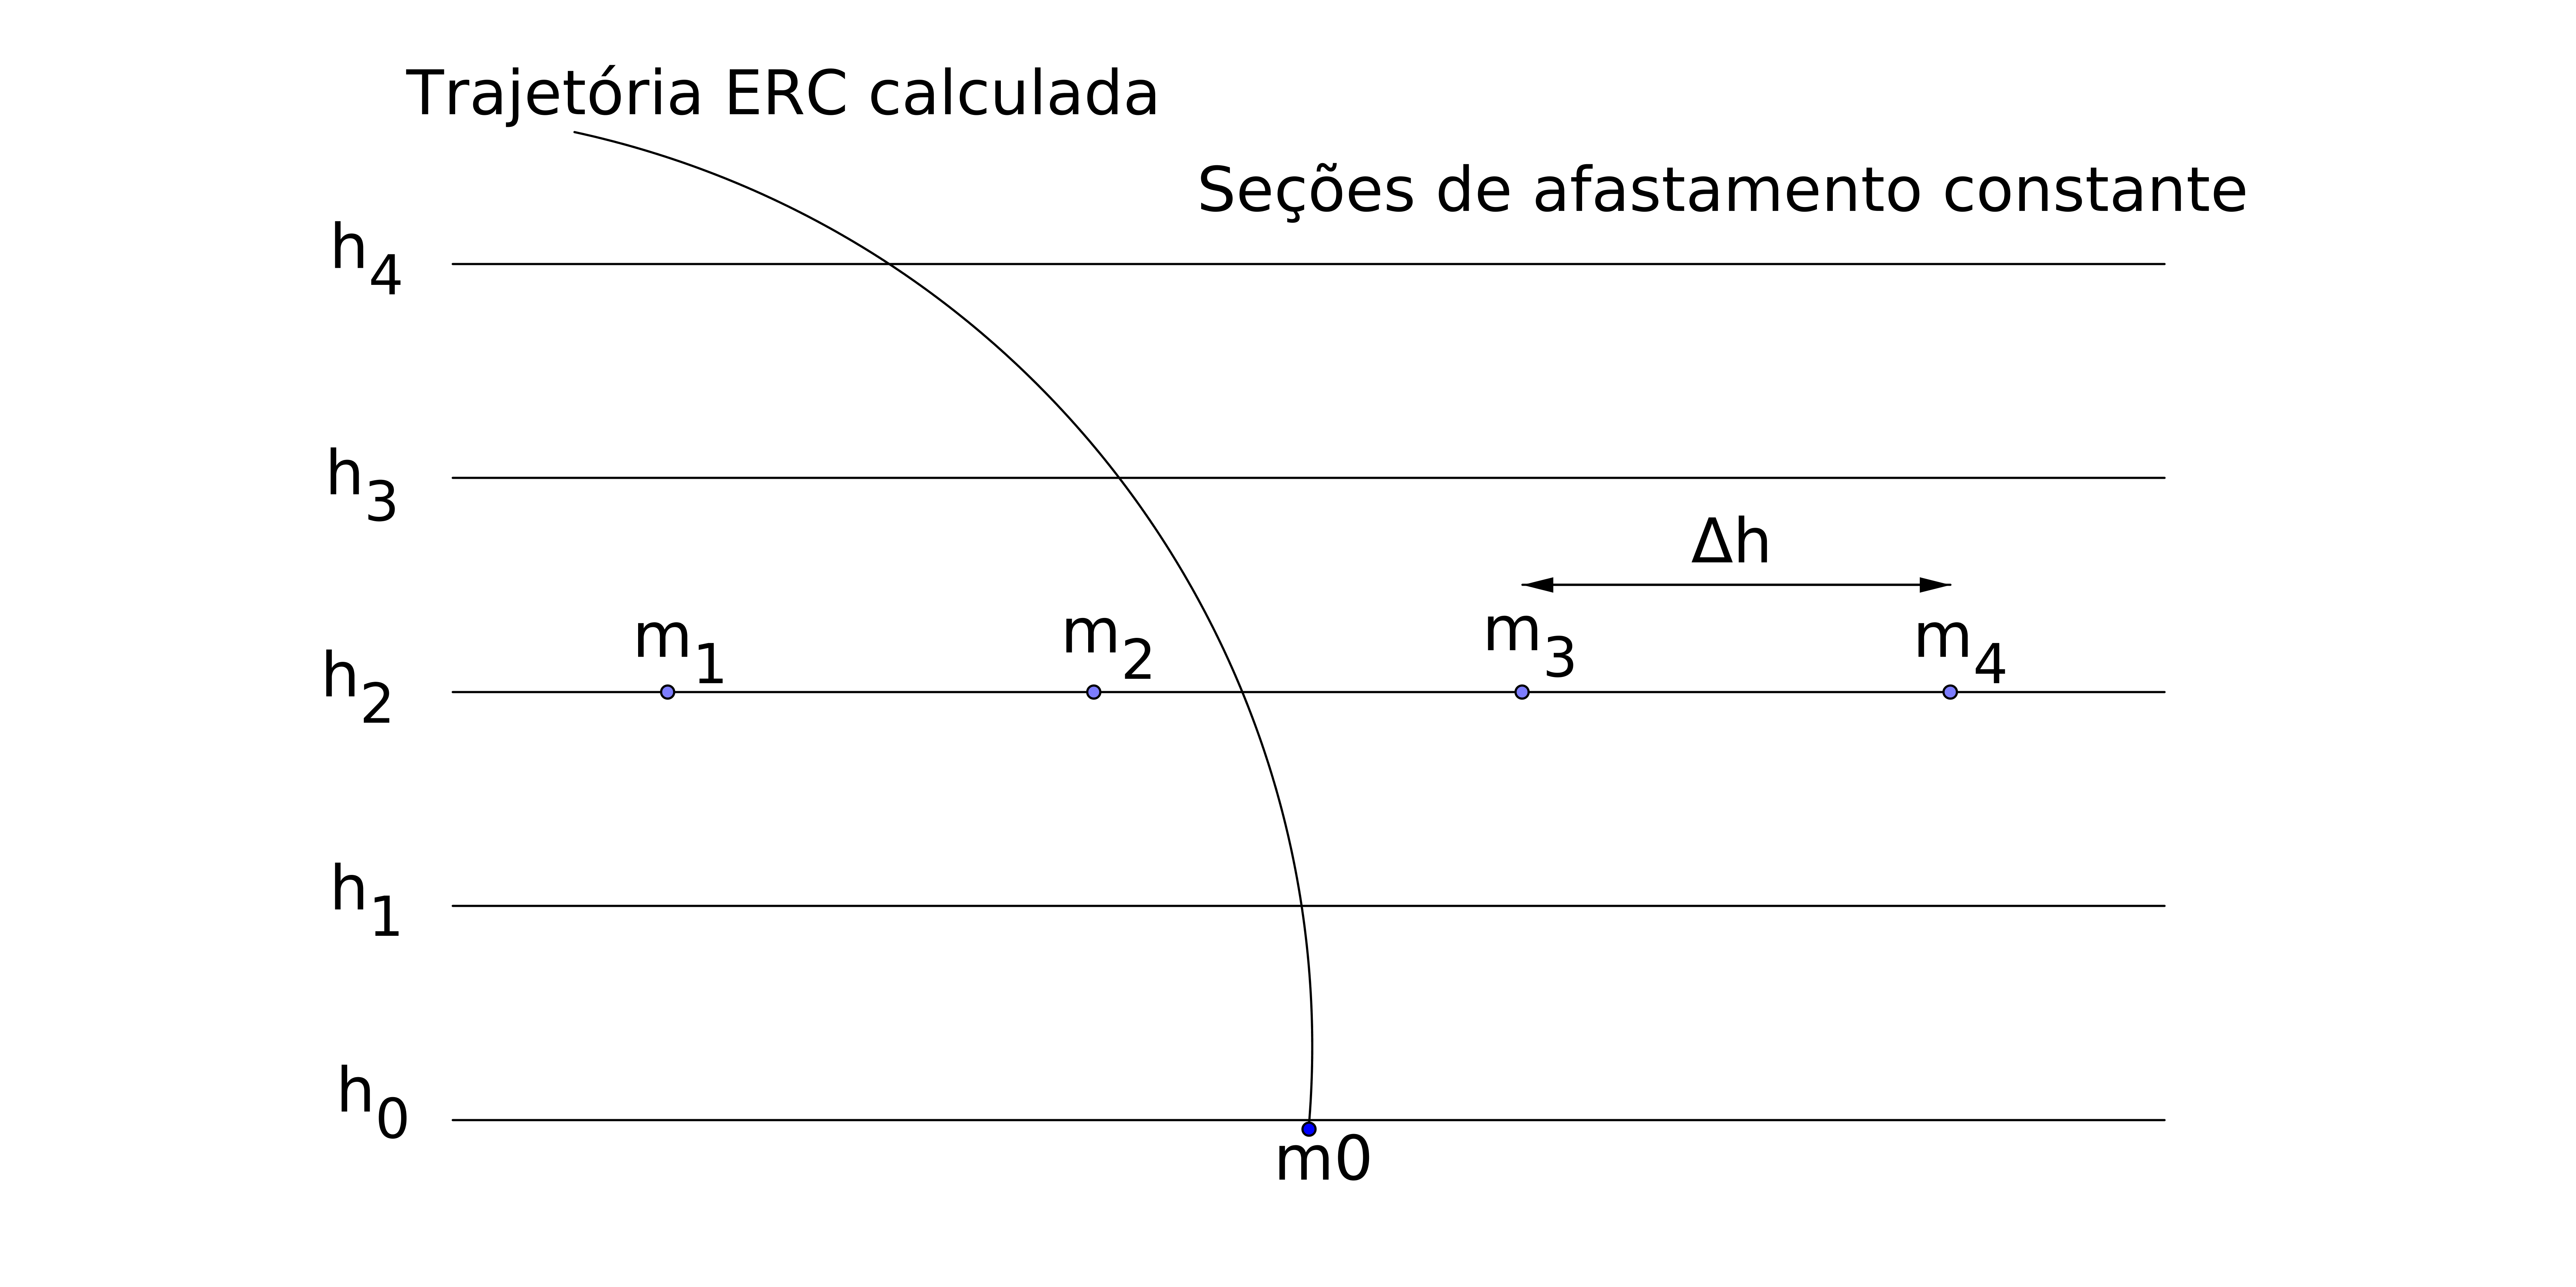
\includegraphics[scale=0.15]{images/interpolacao0.png}
\vspace{-0.3cm}
\end{center}
\begin{center}
 Fonte: Do Autor.
\end{center}
\label{fig:3.1}
\end{figure}


\begin{figure}
\caption{Representação esquemática das seções de afastamento constante após a interpolação. A discretização foi aumentada
intercalando traços zerados $m'_i$ entre os traços originais e depois realizando a interpolação FPE. O traço sísmico 
identificado pela coordenada $m'_2, h2$ está mais próximo da coordenada real da trajetória ERC calculada que os traços 
originais $m_2, h2$ e $m_3, h2$. o processo de interpolação é repetido até que a discretização seja suficiente para amostrar a 
trajetória ERC.}
\begin{center}
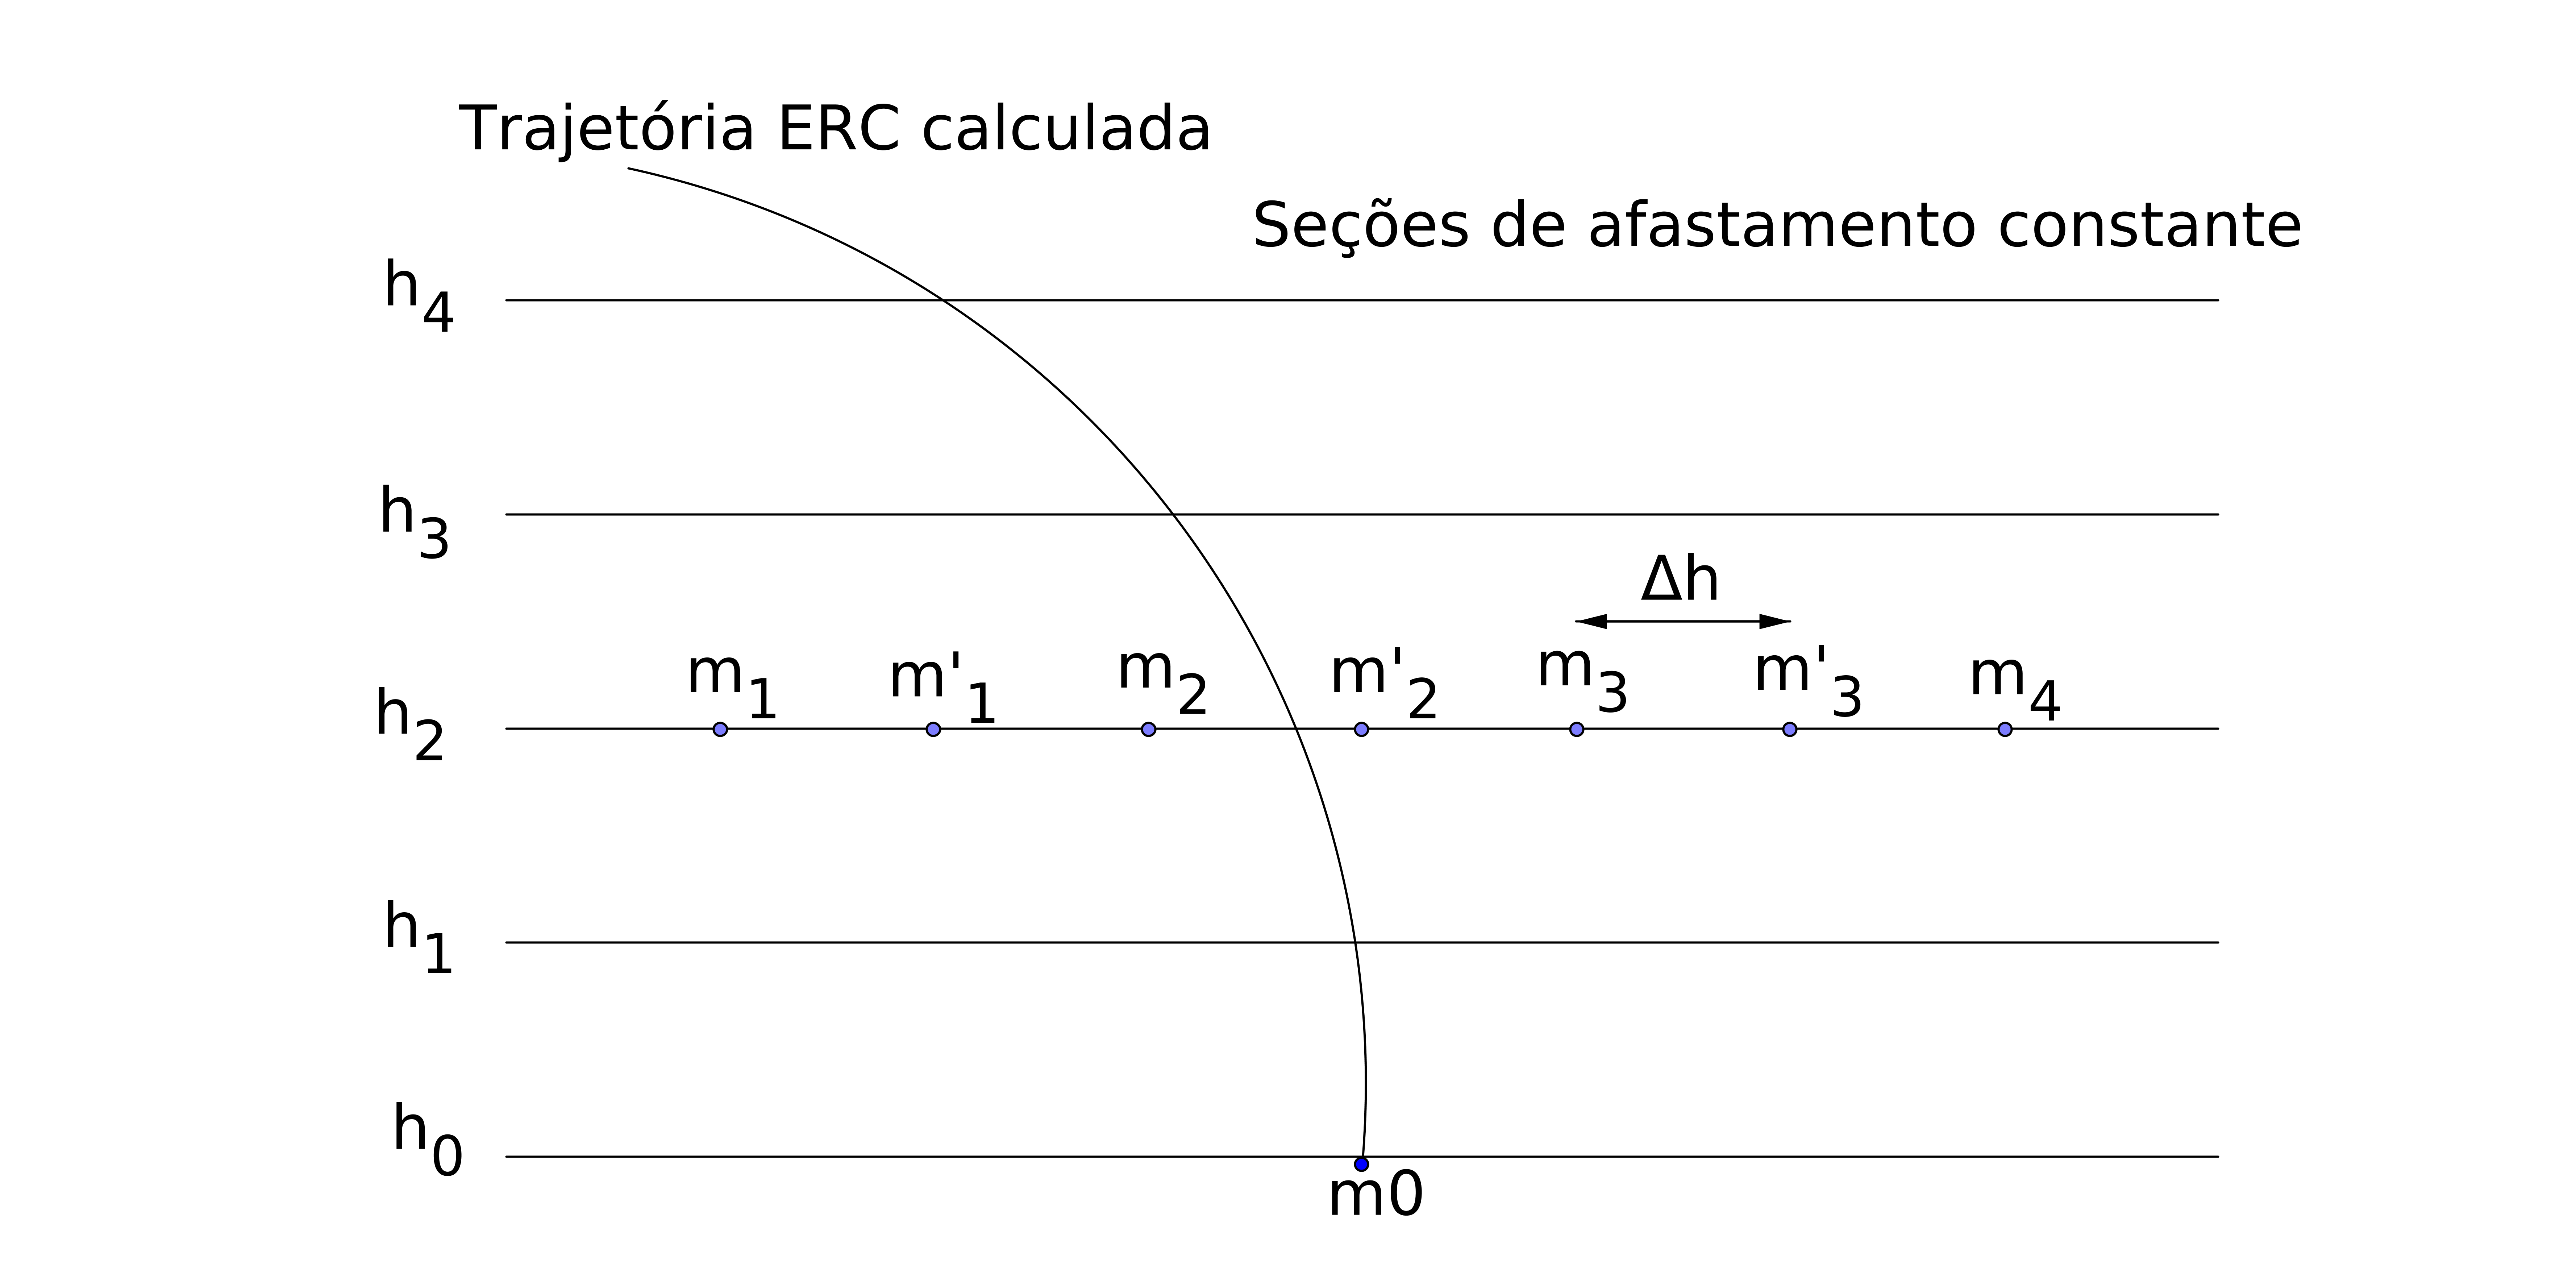
\includegraphics[scale=0.15]{images/interpolacao.png}
\vspace{-0.3cm}
\end{center}
\begin{center}
 Fonte: Do Autor.
\end{center}
\label{fig:3.2}
\end{figure}

